\documentclass[12pt]{article}
%\renewcommand\normalsize{\fontsize{10pt}{12pt}\selectfont}
\usepackage{graphicx} % Required for inserting images
\usepackage[left=2cm,right=2cm,top=2cm,bottom=1.5cm]{geometry}
\usepackage{wrapfig}
 \pagestyle{empty} 

\title{Midterm}
%\author{Dennis Wilkinson}
%\date{March 31 2025; due Monday April 7}

\begin{document}

\setlength{\parindent}{0pt}
\setlength{\parskip}{3mm}
FS1 Wilkinson - Midterm

May 1, 2025

\textbf{1}. Below is the plot of $v$ vs $t$ for a cart on a flat track from physics lab. Let's define positive $v$ to mean eastward motion, and negative westward. The flattish parts in the middle aren't totally flat, because of friction or air resistance.

\begin{figure}[h]
    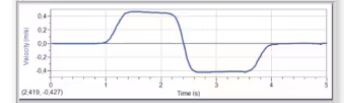
\includegraphics[width=0.6\linewidth]{cart bounce.JPG}
\end{figure}

\textbf{a.} Name a moment in time (in seconds - use the graph) when the velocity was nonzero, but the acceleration was very close to zero. What was the cart doing at this time?

\textbf{b.} When the velocity was briefly 0, at around $t=2.4$ seconds, find the magnitude (approximately) and direction of the acceleration. Use the numbers from the graph.

\textbf{c.} Name all the times when was there a significantly nonzero net force (meaning, not counting the friction/air resistance) on the cart.

\textbf{d.} Describe what must have happened in this lab experiment, and sketch a graph of $x$ vs $t$ for this motion - qualitative only, no numbers required.

\bigskip

\textbf{2.} A solid rubber lacrosse ball and a hollow rubber racquetball are dropped off the roof of the Scarborough building. They have the same air drag coefficient and radius, but the lacrosse ball's mass is greater. 

Explain why \textbf{(a.)} the initial accelerations are identical, but \textbf{(b.)} the lacrosse ball eventually has a larger terminal velocity. On (b), use a free body diagram as part of your explanation. 

\textbf{c.} The lacrosse ball's mass is 150 grams. Consider a time during which the lacrosse ball fell 10 meters at terminal velocity. Find the increase in energy of the air molecules during this time.

\textbf{d.*} Say the lacrosse ball was dropped in an airtight cylindrical silo of radius 5 m and height 20 m at 1 atm and 300 K; and further, the total KE lost in the fall was twice your answer to part (c). The air temperature increases to 300 + $T$; find the order of magnitude (power of ten) of $T$.

\bigskip

\textbf{3.} Venus and Earth have very nearly circular orbits of radius 0.723 AU and 1 AU, respectively.

\textbf{a.} Explain conceptually, or using an equation, why Venus' speed must be larger than Earth's. 

\textbf{b.} Find Venus's total energy (with the usual convention of $U=0$ at $r=\infty$). Use 1 AU = $1.5 \times 10^{11}$ m, $G=6.7 \times 10^{-11}$ Nm$^2$/kg$^2$, $M_{Sun}=2.0 \times 10^{30}$ kg and $M_{Venus}=4.9 \times 10^{24}$ kg.

\textbf{c*.} Imagine that, for some physics-test Deus-ex-machina reason, Venus' speed suddenly changes from $v$ to $v(1+\alpha)$, for some value of $\alpha$. Explain what would happen to the orbit, qualitatively, for the following values of $\alpha$: (i) -0.3; (ii) +0.3; (iii) +0.5. Defend answer for full credit.  

%4. Consider a ball attached to the end of a wooden rod which rotates in a vertical circle, similar to the motion of one cart in a Ferris Wheel. 

%a. If the ball is moving at a constant speed, the rod length is 0.2 meters and it makes one rotation every second, find the ball's speed.

%b. If the mass of the ball is 1 kg, find the tension (or compression) force in the rod at the bottom of the motion, and at the top of the motion - two different answers. If you couldn't solve (a), use $v=1.5$ m/s.

\newpage

\textbf{4.} A refrigerator works like an AC system, transporting heat from inside the fridge out into the room. 

\textbf{a.} Explain how this works, including the purpose of the compressor and the expansion valve.

\textbf{b.} What would happen to the room's temperature if we left the fridge door open (while the fridge was running)? Why?

\textbf{c.} When the coolant fluid passes through the expansion valve, it very quickly goes from a pressure of 100 psi to 35 psi. If the fluid temperature was 100 $^{\circ}$F before the expansion, find the temperature afterwards. Use $\gamma=1.12$.

\bigskip

\textbf{5.} A car goes around a circular bend in the road; friction provides the centripetal force.

\textbf{a.} Using the expression for centripetal force, explain why a car might make it around a certain corner at speed $v$ on a dry day, but spin out at that same speed on a rainy day.

\textbf{b*.} The friction force on the car is proportional to its mass. Explain why, therefore, the speed warning signs (``Slow curve - 25 MPH" or whatever) apply equally to cars regardless of their mass.

\bigskip

\begin{wrapfigure}[10]{l}{0.35\textwidth}
  \centering
    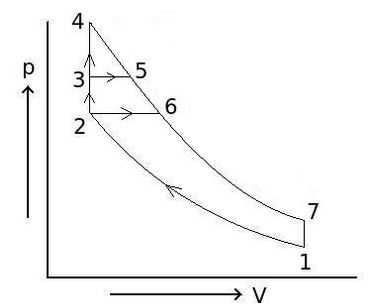
\includegraphics[width=0.35\textwidth]{PV3.JPG}
\end{wrapfigure}

\textbf{6.} The PV diagram to the left shows the (idealized) cycles for three different two-stroke engines: Otto (1-2-4-7), dual (1-2-3-5-7), and Diesel (1-2-6-7).

\textbf{a.} Rank them in terms of the work done per cycle; briefly defend your answer.


\textbf{b.} In step 2-6 of the Diesel cycle, is there $W$ done on the gas, by the gas, or zero? What is the sign of $Q$ and $\Delta U$ in this step? Defend your answer. 

\textbf{c.} Explain, briefly, what is happening during each step of the Diesel cycle. 6-7 and 1-2 are adiabatic.  

%\begin{wrapfigure}[h]{l}{0.5\linewidth}
%    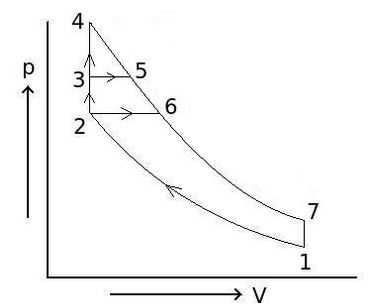
\includegraphics[width=0.3\linewidth]{PV3.JPG}
%\end{wrapfigure}

\begin{wrapfigure}{l}{0.35\textwidth}
  \begin{center}
    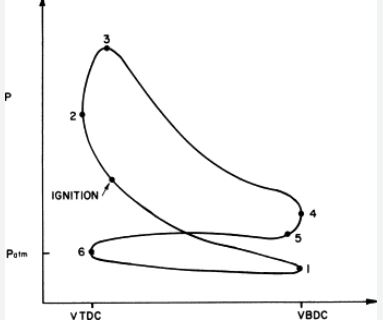
\includegraphics[width=0.35\textwidth]{real otto.JPG}
  \end{center}
\end{wrapfigure}

\bigskip
\bigskip

\textbf{Bonus} The PV diagram to the left is supposed to be close to the actual (not idealized) PV diagram for a four-stroke Otto cycle. 

a. Explain why the line isn't vertical between ignition and 3; what must be happening?
%\begin{figure}[h]
%    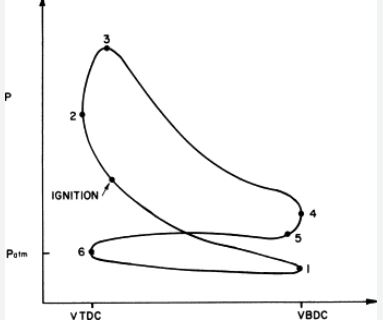
\includegraphics[width=0.27\linewidth]{real otto.JPG}
%\end{figure}
  
b. In the exhaust stroke 5-6-1 of the real four-stroke Otto, are the car wheels losing energy, or gaining it? Why or why not?
 
\end{document}